\documentclass[12pt,a4paper]{article}
\usepackage[utf8]{inputenc}
\usepackage[T1]{fontenc}
\usepackage[brazil]{babel}
\usepackage[margin=2.5cm]{geometry}
\usepackage{booktabs}
\usepackage{amsmath,amssymb}
\usepackage{caption}
\usepackage{graphicx}
\usepackage{setspace}
\usepackage{indentfirst}
\usepackage{longtable}
\usepackage{float}
\usepackage{placeins}
\usepackage{fancyhdr}
\usepackage[hidelinks]{hyperref}
\usepackage[alf]{abntex2cite}

\graphicspath{{v2 OFICIAL/figuras/}}

\captionsetup{font=small,labelsep=colon}
\onehalfspacing
\setcounter{tocdepth}{2}

\pagestyle{fancy}
\fancyhf{}
\fancyhead[L]{\footnotesize Peso de ações nos fundos de investimento brasileiros}
\fancyhead[R]{\footnotesize J. P. Zangrandi}
\fancyfoot[C]{\thepage}
\renewcommand{\headrulewidth}{0.4pt}

\begin{document}

%==================== CAPA ====================
\thispagestyle{empty}
\begin{center}
{\large FUNDAÇÃO GETÚLIO VARGAS}\\[2pt]
{\large ESCOLA DE ECONOMIA DE SÃO PAULO}\\[16pt]
{\normalsize Graduação em Economia}

\vspace{3.5cm}

{\large João Paulo Zangrandi}

\vspace{2.5cm}

{\Large Peso de ações nos fundos de investimento brasileiros:}\\[12pt]
{\large um modelo de fator dinâmico com correção logística e ajuste parcial}

\vspace{2.5cm}

\begin{flushright}
\begin{minipage}{0.62\textwidth}
\small\setstretch{1.15}
Monografia II apresentada à Escola de Economia de São Paulo da Fundação Getúlio
Vargas como requisito da disciplina Monografia II.
\\[10pt]
Orientador: Prof.\ Maurício Ferraresi Junior.
\end{minipage}
\end{flushright}

\vfill

{\normalsize São Paulo}\\
{\normalsize 2026}
\end{center}

\newpage

%==================== RESUMO ====================
\thispagestyle{fancy}
\begin{center}{\large Resumo}\end{center}
\noindent
Este trabalho propõe e testa um modelo de fator dinâmico para o peso de ações na carteira
dos fundos de investimento brasileiros, organizado em três etapas. Na primeira, o peso de
cada fundo em cada ativo é estimado, mês a mês e ativo a ativo, por regressão logística
sobre seis características observáveis do fundo, a saber, o tamanho, o número de cotistas,
a condição de fundo de investimento em cotas, o fluxo de captação líquida sobre o
patrimônio, o beta da cota e a concentração do restante da carteira. Na segunda, um
mecanismo de ajuste parcial modela a velocidade com que a posição observada converge ao
alvo estimado na primeira etapa. Na terceira, o parâmetro de ajuste é reestimado apenas
com os meses anteriores a janeiro de 2020 e aplicado, fixo, ao período seguinte, de modo a
medir o valor preditivo do modelo em dados que ele não viu durante a estimação. A base
cobre todo o universo de fundos da Comissão de Valores Mobiliários com posição em ações
entre 2016 e 2021, do qual resulta uma amostra final de 2.507 fundos, 41 grupos de gestora
e 512 ativos, com 8.212.294 observações de fundo por ativo e por mês. O número de
cotistas, o beta da cota e a concentração do restante da carteira são as características
mais consistentemente associadas ao peso. A velocidade de ajuste estimada é positiva e
pequena, de 0,069 ao mês, e o modelo de ajuste parcial supera a previsão ingênua de
repetir o último peso observado nos quatro horizontes testados, com margem que cresce com
o horizonte. O erro fora da amostra é heterogêneo entre gestoras, e essa heterogeneidade
está associada sobretudo à concentração da carteira, que permanece estatisticamente
significativa mesmo quando as demais características do modelo são controladas.

\smallskip
\noindent Palavras-chave: sistema de demanda; fundos de investimento; pesos de carteira;
fator dinâmico; ajuste parcial; mercado acionário brasileiro.

\newpage
\thispagestyle{fancy}
\tableofcontents
\newpage

%==================== 1. INTRODUÇÃO ====================
\section{Introdução}
\label{sec:introducao}

A composição das carteiras dos fundos de investimento é uma das informações mais ricas e
ao mesmo tempo menos exploradas do mercado de capitais brasileiro. Quando um fundo decide
quanto de cada ação carregar, ele revela, ainda que parcialmente, a sua demanda por aquele
papel. Observar simultaneamente todos os fundos que carregam uma mesma ação equivale,
portanto, a observar um grande conjunto de decisões de demanda tomadas no mesmo mês, sob o
mesmo conjunto de preços, o que torna possível investigar de forma organizada duas
perguntas. A primeira é quais características de um fundo explicam o peso que ele atribui
a uma ação. A segunda é se esse peso pode ser previsto alguns meses à frente, em dados que
o modelo não utilizou para se estimar.

O arcabouço teórico de referência é o sistema de demanda de \citeonline{koijen2019}, que
propõem tratar os preços dos ativos como resultado das demandas de investidores que
escolhem suas carteiras em função de um conjunto reduzido de características. A principal
vantagem dessa abordagem é reduzir um problema de dimensão muito alta, com milhares de
ativos e investidores, a um número pequeno de parâmetros interpretáveis. O presente
trabalho situa-se no lado das quantidades desse programa. Em vez de estimar como a demanda
reage a preços, estima-se como o peso de uma ação reage às características dos fundos que a
carregam. Em linha próxima, \citeonline{gabaix2021} argumentam que os mercados acionários
são pouco elásticos, de modo que fluxos de demanda têm efeito expressivo sobre preços, o
que reforça o interesse em medir diretamente a demanda dos investidores institucionais,
justamente o que as carteiras divulgadas dos fundos permitem observar.

Este trabalho responde às duas perguntas com um modelo de três etapas, detalhado na
Seção~\ref{sec:metodologia}. Na primeira etapa, o peso que cada fundo carrega em cada ação
é modelado por regressão logística sobre seis características do fundo, a saber, o
tamanho, o número de cotistas, a condição de fundo de investimento em cotas, o fluxo de
captação líquida sobre o patrimônio, o beta da cota e a concentração do restante da
carteira. Essa regressão é estimada célula a célula, isto é, separadamente para cada par de
ativo e mês, sem nenhuma agregação temporal por cima, de modo que os coeficientes formam
uma série de cortes transversais que pode ser lida como um fator latente que varia no
tempo, na tradição de \citeonline{famamacbeth1973}. Na segunda etapa, um mecanismo de
ajuste parcial modela a velocidade com que a posição efetivamente observada converge ao
alvo implícito nessas características. Na terceira, o modelo inteiro é submetido a um
teste fora da amostra, com um corte temporal único, contra a referência exigente da
previsão ingênua que apenas repete o último peso observado.

A amostra é ampla e vem inteiramente de registros públicos. Ela parte de todo fundo do
universo da Comissão de Valores Mobiliários que registrou posição em ações entre 2016 e
2021 e chega, depois dos filtros de disponibilidade de característica descritos na
Seção~\ref{sec:dados}, a 2.507 fundos, 41 grupos de gestora e 512 ativos, com 8.212.294
observações de fundo por ativo e por mês. Não se trata, portanto, de um recorte restrito a
uma única gestora ou a uma única ação, o que permite avaliar se os padrões encontrados são
gerais ou peculiares a um caso escolhido.

Os resultados têm três lados. Para explicar o peso, as características funcionam bem, e o
número de cotistas, o beta da cota e a concentração do restante da carteira são as mais
consistentes em sinal ao longo das mais de treze mil células estimadas. Para prever, o
ajuste parcial supera a previsão ingênua nos quatro horizontes testados, com margem que
cresce de forma monotônica com o horizonte, ainda que a velocidade de ajuste estimada seja
pequena, o que indica uma reversão lenta ao peso-alvo definido pelas características e
convive com a forte persistência do peso no curto prazo. Por fim, o erro fora da amostra é
bastante heterogêneo entre gestoras, e essa heterogeneidade não é ruído: ela é persistente
de uma metade do período de teste para a outra, sobretudo na dispersão do erro, e está
associada de forma robusta à concentração da carteira, mesmo depois de controlar as demais
características do modelo.

A contribuição do trabalho é reunir, para o mercado brasileiro e a partir de bases
públicas, uma cadeia completa que costuma aparecer fragmentada na literatura, indo da
característica do fundo ao peso previsto, do peso previsto à dinâmica de ajuste e da
dinâmica de ajuste ao desempenho preditivo fora da amostra. A evidência brasileira sobre
demanda por ativos construída a partir de carteiras de fundos é escassa, e organizar esse
painel de forma reprodutível já é, por si só, parte do que se propõe aqui.

O restante do texto está organizado da seguinte forma. A Seção~\ref{sec:revisao} revisa a
literatura de precificação baseada em demanda, de efeitos de fluxo de fundos e de modelos
de ajuste parcial. A Seção~\ref{sec:dados} descreve as fontes de dado e a construção da
amostra. A Seção~\ref{sec:metodologia} formaliza as três etapas do modelo. A
Seção~\ref{sec:resultados} apresenta os resultados de cada etapa, com ênfase no desempenho
fora da amostra e na heterogeneidade entre gestoras. A Seção~\ref{sec:conclusao} conclui e
registra as limitações do desenho.

%==================== 2. REVISÃO DE LITERATURA ====================
\section{Revisão de literatura}
\label{sec:revisao}

Este trabalho se apoia em três correntes da literatura de finanças que raramente aparecem
juntas no mesmo desenho empírico: a precificação de ativos baseada em demanda, o estudo dos
efeitos de fluxo e de negociação institucional sobre preços, e os modelos de ajuste parcial
aplicados a decisões de carteira. Cada uma contribui com uma peça do modelo de três etapas
descrito na Seção~\ref{sec:metodologia}, e é a combinação delas, aplicada ao mercado
brasileiro a partir de bases públicas, que define o espaço que este trabalho procura ocupar.

A primeira corrente parte da premissa de que a demanda de investidores institucionais por
ativos específicos afeta preços de forma economicamente relevante, e não apenas como ruído
absorvido por arbitradores perfeitamente elásticos. Sua formalização mais completa está em
\citeonline{koijen2019}, que estimam um sistema de demanda a partir das carteiras de
diferentes tipos de investidor institucional americano e mostram que a elasticidade de
demanda observada é ordens de grandeza menor do que modelos sem fricção preveem, de modo que
o rebalanceamento institucional move o preço. \citeonline{gabaix2021} levam o argumento
adiante e propõem a hipótese de mercados inelásticos, segundo a qual um real que entra no
mercado acionário eleva a capitalização agregada em várias vezes esse valor, o que
transforma a medição direta da demanda institucional em objeto de interesse por si só. A
primeira etapa deste trabalho responde a uma versão mais restrita da mesma pergunta, isto é,
o que explica a carteira observada de um fundo em cada ativo e em cada mês, com uma
especificação de corte transversal mais simples do que o sistema de demanda completo, porém
com a mesma lógica de fundo, a de que características observáveis do investidor predizem sua
carteira.

A segunda corrente é anterior e mais extensa, e documenta que a negociação dos fundos, e não
apenas o nível de suas carteiras, move preços. \citeonline{lakonishok1992} estão entre os
primeiros a quantificar o efeito da negociação institucional em bloco sobre o preço e a
propor uma medida de comportamento de manada que se tornou padrão na literatura seguinte, e
\citeonline{wermers1999} aplica essa medida a fundos mútuos americanos e encontra
comportamento de manada moderado, porém concentrado em ações pequenas e de crescimento, com
efeito de preço mensurável nos trimestres seguintes. \citeonline{coval2007} e
\citeonline{edelen2001} deslocam o foco para o mecanismo, mostrando que fundos que sofrem
resgates grandes são forçados a vender posições existentes por razões não relacionadas a
informação sobre o ativo, o que cria pressão de preço que reverte parcialmente, e
\citeonline{lou2012} converte essa ideia em um sinal de retorno esperado ao mostrar que o
fluxo previsto a partir do fluxo passado do fundo e de sua carteira prediz retorno futuro do
ativo. Essa literatura é o que justifica incluir o fluxo de captação líquida entre as
características do modelo, e é também a razão pela qual a interpretação dos resultados da
Seção~\ref{sec:resultados} precisa distinguir com cuidado o que é previsão de carteira do
que seria previsão de preço.

Ainda do lado da demanda, uma literatura complementar mostra quais características de fundo
explicam sistematicamente sua carteira e seu comportamento de negociação.
\citeonline{gompers2001} documentam que a participação institucional em uma ação está
associada ao tamanho da empresa, à liquidez e a características de governança, e que essa
composição de propriedade se desloca ao longo do tempo de forma previsível.
\citeonline{chevalier1997} e \citeonline{sirri1998} estudam o lado dos incentivos, mostrando
que a relação entre desempenho passado e captação é convexa e que os gestores respondem a
ela ajustando o risco da carteira. Essas três referências motivam diretamente a escolha das
seis características empregadas na primeira etapa deste trabalho, que são, em essência, uma
adaptação dessas dimensões ao que o dado público brasileiro permite observar sobre cada
fundo.

A terceira corrente fornece a dinâmica. A ideia de ajuste parcial, segundo a qual um agente
não salta instantaneamente para o seu alvo mas fecha uma fração fixa da distância a cada
período, vem originalmente da literatura de estrutura de capital. \citeonline{fama2002} e
\citeonline{flannery2006} estimam a velocidade com que empresas convergem à sua
alavancagem-alvo e documentam heterogeneidade substancial entre firmas nessa velocidade, um
padrão qualitativo que este trabalho encontra novamente, agora entre gestoras de fundos.
Mais próximo da aplicação aqui, \citeonline{calvet2009} modelam o rebalanceamento de carteira
de investidores individuais suecos como ajuste parcial em direção a um peso-alvo e mostram
que a maioria rebalanceia de forma ativa, porém incompleta e heterogênea. A segunda etapa
deste trabalho transporta esse mecanismo para fundos institucionais brasileiros, com a
diferença de que o alvo não é exógeno, e sim estimado na própria primeira etapa a partir das
características do fundo.

Nenhuma dessas correntes, isoladamente, percorre a cadeia completa que vai da característica
do fundo ao peso previsto, do peso previsto à velocidade de ajuste e desta ao desempenho
preditivo fora da amostra, e menos ainda o faz para o mercado brasileiro. A evidência
nacional sobre demanda por ativos construída a partir de carteiras divulgadas de fundos é
escassa, e é essa lacuna que o desenho descrito a seguir procura preencher.

%==================== 3. DADOS ====================
\section{Dados}
\label{sec:dados}

Os dados vêm de dois registros públicos que a Comissão de Valores Mobiliários exige de todo
fundo de investimento brasileiro. O primeiro é a Composição e Diversificação de Aplicações,
extrato mensal do qual se extrai o peso de cada ativo na carteira de cada fundo, que é a
variável dependente deste trabalho. O segundo é o Informe Diário, do qual vêm o patrimônio
líquido, o número de cotistas, a captação e os resgates, que compõem as características do
fundo. O período coberto vai de janeiro de 2016 a dezembro de 2021. O universo de partida é
todo fundo registrado na Comissão que tenha mantido posição em ações no período, o que
totaliza 3.254 fundos, 41 grupos de gestora reunidos por marca controladora e 536 ativos de
posição direta. Não há, portanto, restrição prévia a uma gestora ou a um ativo específico.

Esse universo bruto já reflete uma limpeza de qualidade de dado. Trinta e quatro observações
de fundo por mês, distribuídas em 23 fundos, apresentam soma de participações superior a
150\% do patrimônio na composição divulgada, o que é um erro de reporte na fonte e não um
resultado deste trabalho, e foram excluídas antes de qualquer outra etapa. O corte em 150\%,
e não em 100\%, é deliberado: fundos das classes Ações Livre e Multimercados Livre
ultrapassam de forma persistente os 100\% por alavancagem legítima, de modo que um corte mais
restritivo eliminaria carteiras válidas junto com os erros de reporte.

Um mesmo ativo pode aparecer na composição sob rótulos diferentes conforme o tipo de
posição, isto é, posição direta, posição cedida ou recebida em empréstimo, e direito de
subscrição. Este trabalho mantém apenas a posição direta, identificada pelo sufixo numérico
do código de negociação segundo a convenção da bolsa, o que resulta nos 536 ativos citados
acima e em 10.818.395 linhas de fundo por ativo e por mês antes dos demais filtros.

Seis características de cada fundo entram no modelo, descritas na
Tabela~\ref{tab:caracteristicas}. Cinco delas são medidas no fechamento do mês anterior ao da
observação, de modo a serem predeterminadas em relação ao peso que se quer explicar. O beta
da cota é a exceção, pois sua janela móvel de 252 pregões termina no fechamento do próprio
mês da observação. Essa escolha não utiliza informação futura, já que o peso e o beta em um
mesmo mês usam dado disponível até o mesmo fechamento, mas introduz uma via de endogeneidade
mecânica que as outras cinco características não têm, uma vez que o retorno da cota do fundo
é função, em parte, das próprias posições que o modelo procura explicar. Esse ponto é
retomado entre as limitações registradas na Seção~\ref{sec:conclusao}.

\begin{table}[h]\centering\small
\caption{As seis características do fundo utilizadas na primeira etapa.}
\label{tab:caracteristicas}
\begin{tabular}{@{}p{2.8cm}p{10.5cm}@{}}
\toprule
Característica & Definição \\
\midrule
Tamanho & Logaritmo do patrimônio líquido \\
Cotistas & Logaritmo do número de cotistas \\
FIC & Indicador igual a um se o fundo é fundo de investimento em cotas \\
Fluxo sobre patrimônio & Captação menos resgates, dividido pelo patrimônio líquido \\
Beta da cota & Covariância do retorno diário da cota com o Ibovespa dividida pela variância
do Ibovespa, em janela móvel de 252 pregões \\
Concentração do resto & Índice de Herfindahl da carteira de ações no fechamento do mês
anterior, excluindo o ativo-alvo, conforme a equação~\eqref{eq:hhi-resto} \\
\bottomrule
\end{tabular}
\caption*{\footnotesize Fonte: elaboração própria a partir de dados da Comissão de Valores
Mobiliários. A concentração do resto é calculada sobre o subportfólio de ações capturado no
painel, e não sobre o patrimônio inteiro do fundo, que pode conter renda fixa e caixa não
observados aqui. Fundos sem dado de carteira no mês anterior ficam sem essa característica,
o que corresponde a 2,4\% das linhas.}
\end{table}

A exigência de que as seis características estejam disponíveis linha a linha reduz o
universo bruto de forma sensível, como mostra a Tabela~\ref{tab:universo}. Dos 678 fundos do
universo bruto que não chegam à amostra de cinco características completas, 68 nunca têm as
quatro variáveis do Informe Diário simultaneamente disponíveis, e os outros 610 têm essas
quatro mas nunca chegam a ter beta. Desses 610, a grande maioria, 558 fundos ou 91,5\%,
simplesmente não acumula 252 dias de cota válida dentro da janela de 2016 a 2021, o que
reflete fundos jovens demais e não uma limitação do dado. Os 52 restantes acumulam o
histórico mas não geram beta por outro motivo, como uma janela sem par completo com o
Ibovespa ou o encerramento do fundo logo em seguida.

\begin{table}[h]\centering\small
\caption{Funil da amostra, do universo bruto à amostra final.}
\label{tab:universo}
\begin{tabular}{@{}p{7.6cm}rrr@{}}
\toprule
Etapa & Fundos & Ativos & Gestoras \\
\midrule
Universo bruto com posição em ações, 2016 a 2021 & 3.254 & 536 & 41 \\
Com as cinco características do Informe Diário completas & 2.576 & 513 & 41 \\
Com a concentração do resto defasada disponível & 2.507 & 512 & 41 \\
\bottomrule
\end{tabular}
\caption*{\footnotesize Fonte: elaboração própria a partir de dados da Comissão de Valores
Mobiliários. A cobertura temporal da amostra final é de 59 meses, entre fevereiro de 2017 e
dezembro de 2021, e não os 72 meses do período bruto, porque a exigência de 252 pregões de
histórico de cota para o cálculo do beta elimina os primeiros meses da janela.}
\end{table}

A amostra final resultante, resumida na Tabela~\ref{tab:amostra}, é a base única utilizada
do início ao fim deste trabalho, tanto na estimação quanto no exercício fora da amostra.

\begin{table}[h]\centering\small
\caption{Dimensões da amostra final.}
\label{tab:amostra}
\begin{tabular}{@{}lr@{}}
\toprule
Observações de fundo por ativo e por mês & 8.212.294 \\
Fundos & 2.507 \\
Grupos de gestora & 41 \\
Ativos em posição direta & 512 \\
Meses, de fevereiro de 2017 a dezembro de 2021 & 59 \\
\bottomrule
\end{tabular}
\caption*{\footnotesize Fonte: elaboração própria a partir de dados da Comissão de Valores
Mobiliários.}
\end{table}

\FloatBarrier

%==================== 4. METODOLOGIA ====================
\section{Metodologia}
\label{sec:metodologia}

O trabalho é organizado em três etapas sequenciais, cada uma alimentando a seguinte. A
primeira estima, mês a mês, o peso que cada fundo deveria carregar em cada ativo dadas as
suas características observáveis. A segunda modela a velocidade com que o peso efetivamente
observado converge a esse alvo. A terceira testa, em dados que o modelo não viu durante a
estimação, se essa modelagem tem valor preditivo genuíno. Em todas elas o erro é o principal
objeto de análise, porque é a sua estrutura, isto é, quem erra mais, quando e em que
direção, que permite comparar fundos e gestoras entre si.

\subsection{Primeira etapa: o corte transversal}

Para cada ativo $n$ e cada mês $t$, o peso que um fundo $i$ carrega é modelado como função
logística de suas seis características:
\begin{equation}
\text{peso}_{i,n,t} = g\big(x_{i,n,t}'\theta_{n,t}\big) + e_{i,n,t}, \qquad
g(z) = \frac{1}{1+e^{-z}}
\label{eq:cs}
\end{equation}
em que $x_{i,n,t}$ reúne as seis características descritas na Seção~\ref{sec:dados}, todas
padronizadas com exceção do indicador de fundo de cotas e do fluxo sobre o patrimônio. A
forma logística é adotada porque o peso é limitado ao intervalo entre zero e um, e uma
especificação linear produziria previsões fora desse intervalo justamente nas posições mais
concentradas, que são as economicamente mais interessantes.

O vetor $\theta_{n,t}$ reúne os coeficientes daquele ativo naquele mês e é estimado por
máxima verossimilhança quase-binomial, separadamente para cada célula de ativo e mês que
tenha um número mínimo de fundos detentores, sem nenhuma etapa de agregação temporal por
cima. Cada $\theta_{n,t}$ é, portanto, o resultado de uma única regressão de corte
transversal, e a sequência desses coeficientes ao longo do tempo é o que se lê como fator
dinâmico, no espírito do procedimento de \citeonline{famamacbeth1973}.

A sexta característica exige uma definição explícita, porque envolve o próprio peso que se
quer explicar:
\begin{equation}
\text{HHI}_{\text{resto},i,n,t} = \text{HHI}_{\text{total},i,t-1} - \text{peso}_{i,n,t-1}^2,
\qquad \text{HHI}_{\text{total},i,t-1} = \sum_{m} \text{peso}_{i,m,t-1}^2
\label{eq:hhi-resto}
\end{equation}
Ela mede a concentração da carteira de ações do fundo no fechamento do mês anterior,
excluindo o peso que o próprio ativo-alvo tinha naquele mesmo fechamento. Excluir o
ativo-alvo evita a circularidade de usar como variável explicativa uma medida de
concentração que já incorpora o peso que se está tentando explicar, e defasar a medida para
o mês anterior garante a mesma disciplina de predeterminação das demais características.

O erro dessa etapa, $e_{i,n,t} = \text{peso}_{i,n,t} - g(x_{i,n,t}'\theta_{n,t})$, mede o
quanto a posição observada de um fundo se afasta do que as suas próprias características
explicam, dentro do mesmo mês. Por construção da máxima verossimilhança, a média desse erro
é mecanicamente nula em cada célula, o que não é evidência de bom ajuste e sim uma
propriedade algébrica do estimador. O que de fato varia entre fundos, e é informativo, é a
sua dispersão.

\subsection{Segunda etapa: o ajuste parcial}

A primeira etapa estima um alvo, $w^*_{i,n,t} = g(x_{i,n,t}'\theta_{n,t})$, mas nada diz
sobre a dinâmica, isto é, sobre a rapidez com que a posição real converge a esse alvo. A
segunda etapa modela essa dinâmica por um mecanismo de ajuste parcial, no qual o fundo fecha
a cada mês uma fração $\lambda$ da distância entre a sua posição atual e o alvo:
\begin{equation}
w_{i,n,t+1} - w_{i,n,t} = \lambda\, d_{i,n,t} + u_{i,n,t+1}, \qquad
d_{i,n,t} \equiv w^*_{i,n,t} - w_{i,n,t}
\label{eq:pa}
\end{equation}
O parâmetro $\lambda$ é estimado por mínimos quadrados ordinários sem intercepto, com todos
os pares de meses consecutivos agrupados, de modo a produzir um único coeficiente, ou seja,
a mesma velocidade de ajuste para todo fundo e todo ativo. A meia-vida implícita desse
processo, dada por $\ln(0{,}5)/\ln(1-\lambda)$, traduz o coeficiente em uma unidade mais
interpretável, a saber, quantos meses um fundo leva para percorrer metade da distância até o
seu peso-alvo.

\subsection{Terceira etapa: o exercício fora da amostra}

As duas primeiras etapas são estimadas com a amostra inteira e, por isso, não informam se o
modelo tem valor preditivo genuíno. A terceira etapa testa exatamente isso, com um corte
temporal único. O parâmetro $\lambda_h$, para cada horizonte $h$, é reestimado utilizando
apenas os meses de treino, anteriores a janeiro de 2020, e em seguida aplicado, fixo, aos
meses de teste, de janeiro de 2020 em diante, período que o modelo não viu durante a
estimação:
\begin{align}
\widehat w_{i,n,t+h} &= w_{i,n,t} + \widehat\lambda_{h,\text{treino}}\, d_{i,n,t}
&&\text{(ajuste parcial)} \notag\\
\widehat w_{i,n,t+h} &= w_{i,n,t} &&\text{(previsão ingênua)}
\label{eq:oos}
\end{align}
O erro fora da amostra, definido como $\text{erro}_{i,n,t+h} = \big(w_{i,n,t+h}-w_{i,n,t}\big)
- \widehat\lambda_{h,\text{treino}}\, d_{i,n,t}$, é comparado ao erro da previsão ingênua,
que simplesmente assume que nada muda, por meio da raiz do erro quadrático médio. A diferença
percentual entre as duas raízes, chamada aqui de margem, responde à pergunta central deste
exercício: o ajuste parcial estimado com dados antigos ainda ajuda a prever dados novos, ou
uma previsão ingênua seria igualmente boa? O critério é exigente de propósito, porque o peso
de carteira é uma variável muito persistente, e a regra de repetir o último valor observado
é, nesse contexto, um adversário difícil de bater.

%==================== 5. RESULTADOS ====================
\section{Resultados}
\label{sec:resultados}

Toda esta seção usa a base final descrita na Tabela~\ref{tab:amostra}. A primeira etapa é
estimada célula a célula, com exigência mínima de quinze fundos detentores por célula. Com o
corte de qualidade de dado descrito na Seção~\ref{sec:dados}, o único fundo do grupo Legacy
Capital passa a contribuir com exatamente uma célula, em dezembro de 2021, o que é
insuficiente para que ele apareça em qualquer tabela desta seção que agregue por gestora ao
longo do tempo, já que a segunda e a terceira etapas exigem pares de meses consecutivos. A
base efetivamente estimada é, portanto, de 2.504 fundos, 41 grupos de gestora, 430 ativos com
ao menos uma célula estimada e 8.195.278 observações.

\subsection{Primeira etapa: o que explica o peso}

O modelo da equação~\eqref{eq:cs} foi estimado em 13.723 células de ativo e mês que
convergiram, sendo excluídas outras 17 que não convergiram. A Tabela~\ref{tab:theta} resume,
entre essas células, o coeficiente padronizado de cada característica, o seu efeito marginal
médio em pontos percentuais de peso, e a proporção de células em que o sinal é positivo.

\begin{table}[h]\centering\small
\caption{Coeficiente, efeito marginal médio e consistência de sinal de cada característica,
entre as 13.723 células de ativo e mês estimadas.}
\label{tab:theta}
\begin{tabular}{@{}lrrr@{}}
\toprule
Característica & Mediana do coeficiente & Efeito marginal médio & Células com sinal positivo \\
\midrule
Tamanho & $-0{,}0283$ & $-0{,}0007$ p.p. & $44{,}5\%$ \\
Cotistas & $0{,}1254$ & $0{,}0141$ p.p. & $72{,}8\%$ \\
Fundo de cotas & $-0{,}0244$ & $-0{,}0005$ p.p. & $48{,}3\%$ \\
Fluxo sobre patrimônio & $0{,}0372$ & $0{,}0027$ p.p. & $53{,}0\%$ \\
Beta da cota & $0{,}7830$ & $0{,}1401$ p.p. & $88{,}2\%$ \\
Concentração do resto & $0{,}4220$ & $0{,}0562$ p.p. & $87{,}6\%$ \\
\bottomrule
\end{tabular}
\caption*{\footnotesize Fonte: elaboração própria a partir de dados da Comissão de Valores
Mobiliários. O coeficiente é medido em log-odds sobre a característica padronizada. O
pseudo-$R^2$ de McFadden médio entre as células é de $0{,}531$, calculado com piso em $-1$
para que células mal ajustadas não dominem a média.}
\end{table}

O padrão é claro e tem leitura econômica direta. O beta da cota e a concentração do resto da
carteira são, com folga, as características mais consistentes, com sinal positivo em 88,2\% e
87,6\% das células respectivamente. Um fundo mais exposto ao mercado carrega mais de qualquer
ação dada, o que é o esperado, e um fundo que já concentrava a sua carteira no mês anterior
tende a concentrar também no ativo-alvo neste mês, o que sugere que a concentração é um traço
de estilo do fundo e não uma decisão tomada ativo a ativo. A concentração do resto é
estatisticamente significativa em 74,4\% das células, ou 10.210 das 13.723, e nessas células
o sinal é positivo em 95,7\% dos casos. O número de cotistas vem em seguida, com sinal
positivo em 72,8\% das células, ao passo que o tamanho, a condição de fundo de cotas e o
fluxo sobre o patrimônio ficam próximos do sorteio, com proporções entre 44\% e 53\%. Vale
notar que tamanho e número de cotistas apontam em direções opostas, o que é coerente com a
leitura de que fundos de varejo pulverizados e fundos grandes de poucos investidores são
objetos distintos, ainda que ambos apareçam como grandes pelo patrimônio.

O erro dessa etapa, resumido na Tabela~\ref{tab:erro-e}, tem média nula por construção, como
antecipado na Seção~\ref{sec:metodologia}, e uma dispersão de 0,0117. A assimetria e a
curtose muito altas não são um defeito do ajuste, e sim consequência de a base reunir 512
ativos de liquidez e perfil muito diferentes numa única distribuição agregada, dominada por
posições pequenas e residuais e por algumas poucas concentrações extremas. Nenhuma das
8.195.278 previsões cai fora do intervalo entre zero e um, o que confirma a adequação da
forma funcional escolhida.

\begin{table}[h]\centering\small
\caption{Estatísticas do erro da primeira etapa, em 8.195.278 observações.}
\label{tab:erro-e}
\begin{tabular}{@{}lr@{}}
\toprule
Estatística & Valor \\
\midrule
Média & $0{,}000000$ \\
Desvio-padrão & $0{,}0117$ \\
Mediana & $-0{,}0004$ \\
Mínimo e máximo & $-0{,}688$ e $0{,}985$ \\
Observações com erro positivo & $25{,}4\%$ \\
Assimetria & $11{,}96$ \\
Curtose & $774{,}47$ \\
Previsões fora do intervalo de zero a um & $0$ \\
\bottomrule
\end{tabular}
\caption*{\footnotesize Fonte: elaboração própria a partir de dados da Comissão de Valores
Mobiliários. A curtose de uma distribuição normal é igual a três.}
\end{table}

\FloatBarrier
\subsection{Segunda etapa: a velocidade de ajuste}

O parâmetro da equação~\eqref{eq:pa}, estimado por mínimos quadrados ordinários agrupados
sobre todos os 7.444.169 pares de meses consecutivos da amostra, é $\widehat\lambda =
0{,}0690$. A leitura econômica é que um fundo fecha, em média, apenas cerca de 6,9\% da
distância que o separa do seu peso-alvo a cada mês, o que corresponde a uma meia-vida de
aproximadamente 9,7 meses. Trata-se de um ajuste positivo, portanto na direção prevista pelo
modelo, porém lento, e é justamente essa lentidão que explica a forte persistência do peso no
curto prazo. O padrão qualitativo, de ajuste positivo mas incompleto, é o mesmo que
\citeonline{flannery2006} documentam para a alavancagem das empresas e que
\citeonline{calvet2009} encontram no rebalanceamento de carteiras de investidores
individuais, ainda que os contextos e as unidades de tempo não permitam comparação numérica
direta.

\begin{table}[h]\centering\small
\caption{Estatísticas do erro da segunda etapa, em 7.444.169 pares de meses consecutivos.}
\label{tab:erro-u}
\begin{tabular}{@{}lr@{}}
\toprule
Estatística & Valor \\
\midrule
Média & $-0{,}00004$ \\
Desvio-padrão & $0{,}0045$ \\
Mediana & $0{,}0000$ \\
Mínimo e máximo & $-0{,}892$ e $0{,}592$ \\
Observações com erro positivo & $33{,}4\%$ \\
Assimetria & $-1{,}48$ \\
Curtose & $892{,}04$ \\
\bottomrule
\end{tabular}
\caption*{\footnotesize Fonte: elaboração própria a partir de dados da Comissão de Valores
Mobiliários.}
\end{table}

\FloatBarrier
\subsection{Terceira etapa: desempenho fora da amostra e heterogeneidade}

A Tabela~\ref{tab:oos-agregado} traz o resultado central do trabalho. Com o parâmetro
estimado apenas no período de treino e aplicado fixo ao período de teste, o modelo de ajuste
parcial supera a previsão ingênua nos quatro horizontes examinados, e a vantagem cresce de
forma monotônica com o horizonte, indo de 1,5\% de redução da raiz do erro quadrático médio
em um mês para 7,1\% em doze meses. O parâmetro estimado também cresce com o horizonte, de
0,0704 para 0,3382, o que é exatamente o esperado, pois quanto mais tempo se concede, maior a
fração da distância até o alvo que o fundo consegue percorrer.

\begin{table}[h]\centering\small
\caption{Raiz do erro quadrático médio fora da amostra, ajuste parcial e previsão ingênua,
em quatro horizontes.}
\label{tab:oos-agregado}
\begin{tabular}{@{}lrrrr@{}}
\toprule
& $h=1$ & $h=3$ & $h=6$ & $h=12$ \\
\midrule
Ajuste parcial & $0{,}004033$ & $0{,}005850$ & $0{,}007097$ & $0{,}008546$ \\
Previsão ingênua & $0{,}004095$ & $0{,}006040$ & $0{,}007454$ & $0{,}009198$ \\
Razão entre as duas & $0{,}9849$ & $0{,}9685$ & $0{,}9521$ & $0{,}9291$ \\
Parâmetro de ajuste estimado & $0{,}0704$ & $0{,}1473$ & $0{,}2205$ & $0{,}3382$ \\
\bottomrule
\end{tabular}
\caption*{\footnotesize Fonte: elaboração própria a partir de dados da Comissão de Valores
Mobiliários. O parâmetro é estimado somente com os meses anteriores a janeiro de 2020 e
aplicado, fixo, ao período de janeiro de 2020 a dezembro de 2021.}
\end{table}

A vantagem não se concentra em poucos meses favoráveis. A Figura~\ref{fig:margem-mensal}
mostra a margem mês a mês ao longo de todo o período de teste, com média de 1,48\% no
horizonte de um mês e de 3,13\% no de três meses, e o ajuste parcial vence a previsão ingênua
em todos os 23 meses de teste. Uma checagem adicional confirma que o resultado não depende de
fixar o parâmetro no treino: reestimá-lo mês a mês em janela expansiva, sem utilizar
informação futura, praticamente não altera nada, pois a razão entre as raízes passa de 0,9848
para 0,9849 no horizonte de um mês, ambas as versões vencem a ingênua nos 23 meses, e a
correlação de postos entre os rankings de dificuldade por gestora produzidos pelas duas
versões é igual a um.

\begin{figure}[H]\centering
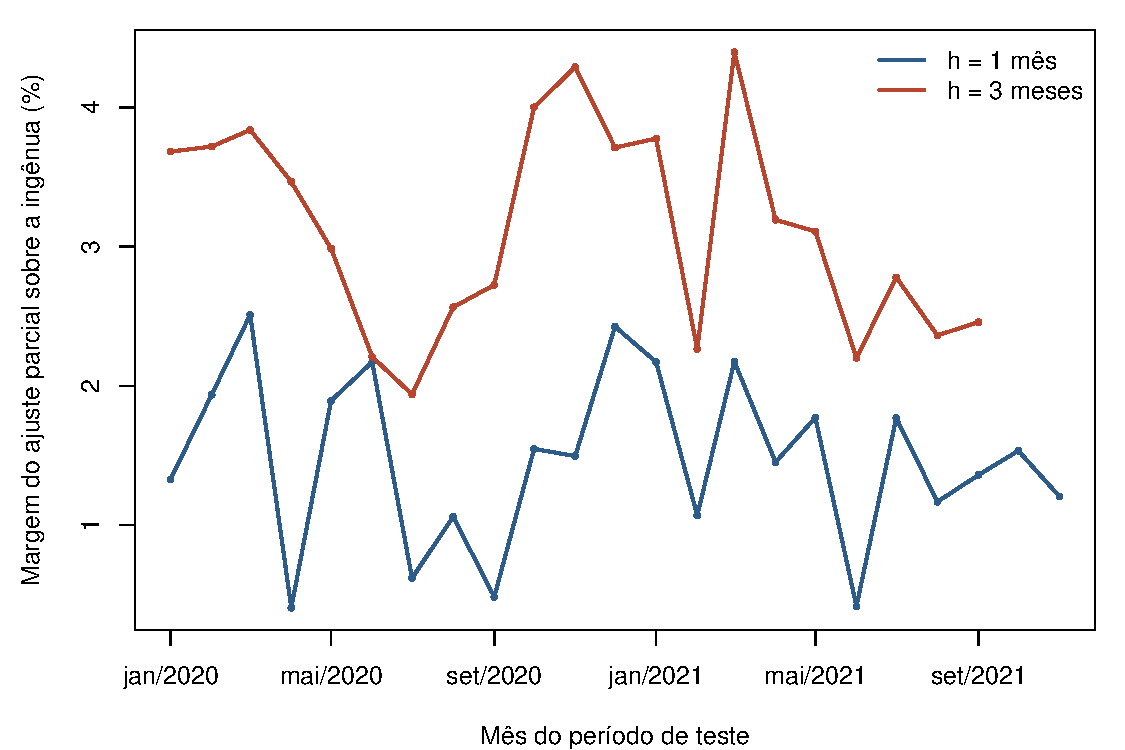
\includegraphics[width=0.75\textwidth]{fig_margem_dinamica_mensal.pdf}
\caption{Margem do ajuste parcial sobre a previsão ingênua, mês a mês, no período de teste.
Fonte: elaboração própria a partir de dados da Comissão de Valores Mobiliários.}
\label{fig:margem-mensal}
\end{figure}

\FloatBarrier

O resultado agregado, contudo, esconde uma heterogeneidade grande entre gestoras. As
Tabelas~\ref{tab:rmse-gestora} e~\ref{tab:margem-gestora} trazem, respectivamente, o erro e a
margem de cada um dos 40 grupos de gestora com dado suficiente, ordenados do mais ao menos
errante no horizonte de um mês. A distância entre os extremos é de quase trinta vezes, indo
de 0,00050 para o grupo Plural a 0,01424 para a Guepardo Investimentos. A leitura conjunta
das duas tabelas mostra que erro alto e margem baixa não são a mesma coisa: há gestoras
difíceis de prever para as quais o ajuste parcial ainda ajuda bastante, como a AZ Quest, com
margem de 15,1\% no horizonte de doze meses, e há gestoras em que o modelo piora a previsão,
sendo a Squadra Investimentos o caso mais extremo, com margem de menos 45,6\% no mesmo
horizonte. A Figura~\ref{fig:erro-extremos} acompanha a evolução mensal do erro nos dois
extremos dessa distribuição.

\begin{figure}[H]\centering
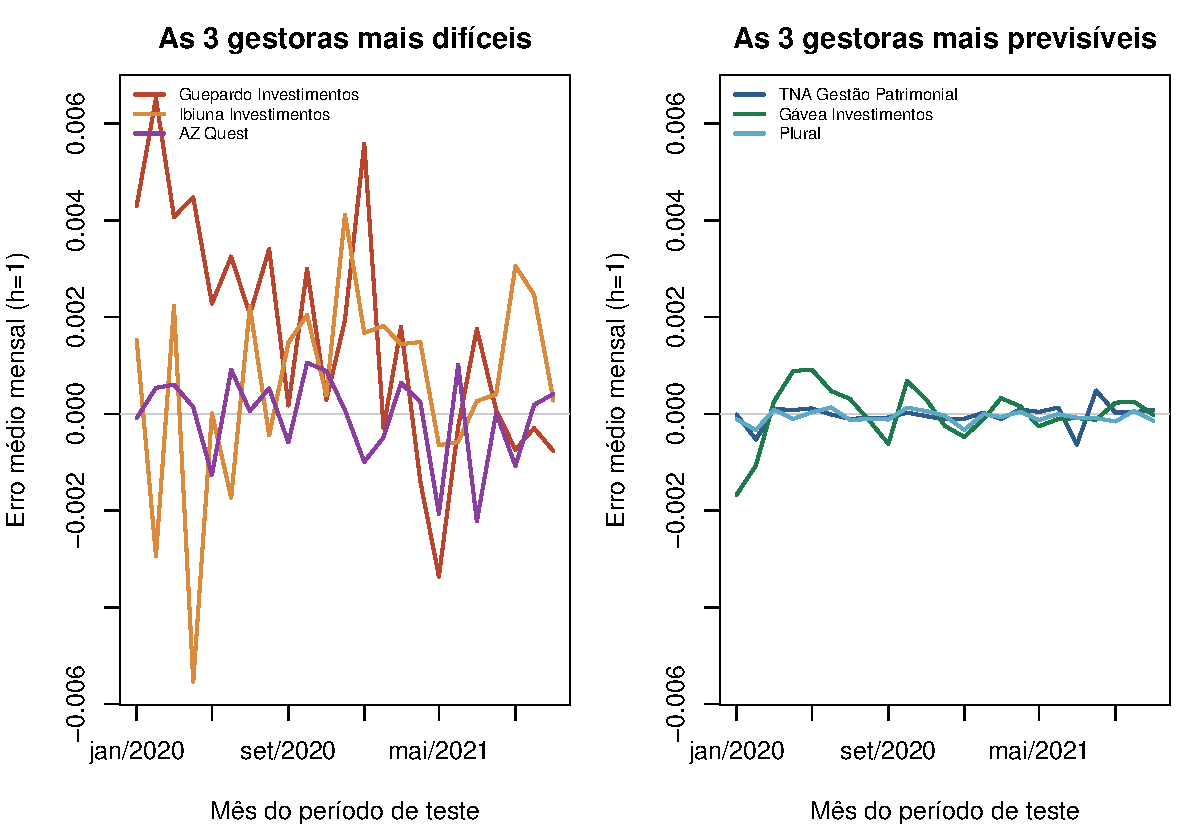
\includegraphics[width=0.95\textwidth]{fig_dinamica_erro_gestora_extremos.pdf}
\caption{Evolução mensal do erro médio fora da amostra no horizonte de um mês, para as três
gestoras de maior e as três de menor erro. Fonte: elaboração própria a partir de dados da
Comissão de Valores Mobiliários.}
\label{fig:erro-extremos}
\end{figure}

\FloatBarrier

O caso da Squadra Investimentos merece exame, porque é o único em que o ajuste parcial piora
a previsão de forma expressiva e crescente com o horizonte. A Figura~\ref{fig:trajetoria}
mostra a trajetória do par de fundo e ativo responsável pelo maior erro de toda a amostra,
uma posição em Equatorial Energia que se mantém entre 97\% e 99,9\% do patrimônio ao longo de
todo o período de teste. Diante de uma concentração desse tamanho, o modelo prevê
repetidamente uma reversão em direção ao alvo que as características implicam, reversão que
nunca acontece, e o erro se acumula a cada horizonte mais longo. O episódio ilustra bem o
limite do desenho: um mandato de fundo que é, por construção, um veículo de posição única não
é capturado por características que descrevem fundos diversificados.

\begin{figure}[H]\centering
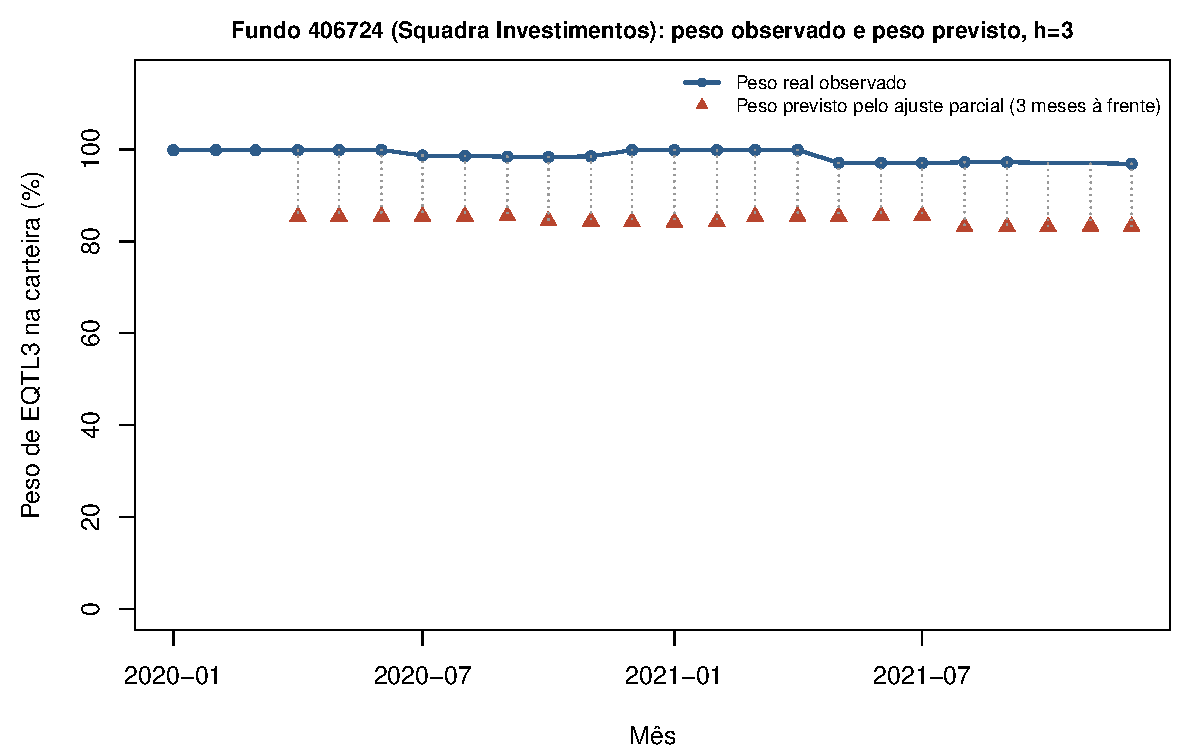
\includegraphics[width=0.78\textwidth]{fig_trajetoria_fundo_pior_rmse.pdf}
\caption{Peso observado e peso previsto no horizonte de três meses para o par de fundo e
ativo de maior erro fora da amostra entre os que mantêm posição relevante. Fonte: elaboração
própria a partir de dados da Comissão de Valores Mobiliários.}
\label{fig:trajetoria}
\end{figure}

\FloatBarrier

A heterogeneidade entre gestoras é estável, e não ruído amostral. Dividindo os 23 meses de
teste ao meio e comparando cada gestora consigo mesma nas duas metades, a correlação do viés
médio é de 0,73, e a do desvio-padrão do erro é de 0,85, valor bem mais alto, ilustrado na
Figura~\ref{fig:persistencia-dp}. Em outras palavras, quem é difícil de prever numa metade do
período de teste tende a continuar difícil na outra, e essa persistência é bastante mais
estável na dispersão do erro do que na sua direção. Isso tem consequência prática: uma
tentativa de correção de viés, estimando o desvio médio de cada gestora na primeira metade e
aplicando-o fixo à segunda, reduz a raiz do erro quadrático médio de 0,005858 para 0,005856,
uma melhora de 0,04\% que é irrelevante. A decomposição do erro confirma o diagnóstico, pois
o quadrado do viés responde, em média entre as gestoras, por apenas 0,46\% do erro quadrático
total, e por praticamente nada quando todas as observações são agrupadas. A variância domina,
e é ela que precisa ser explicada.

\begin{figure}[H]\centering
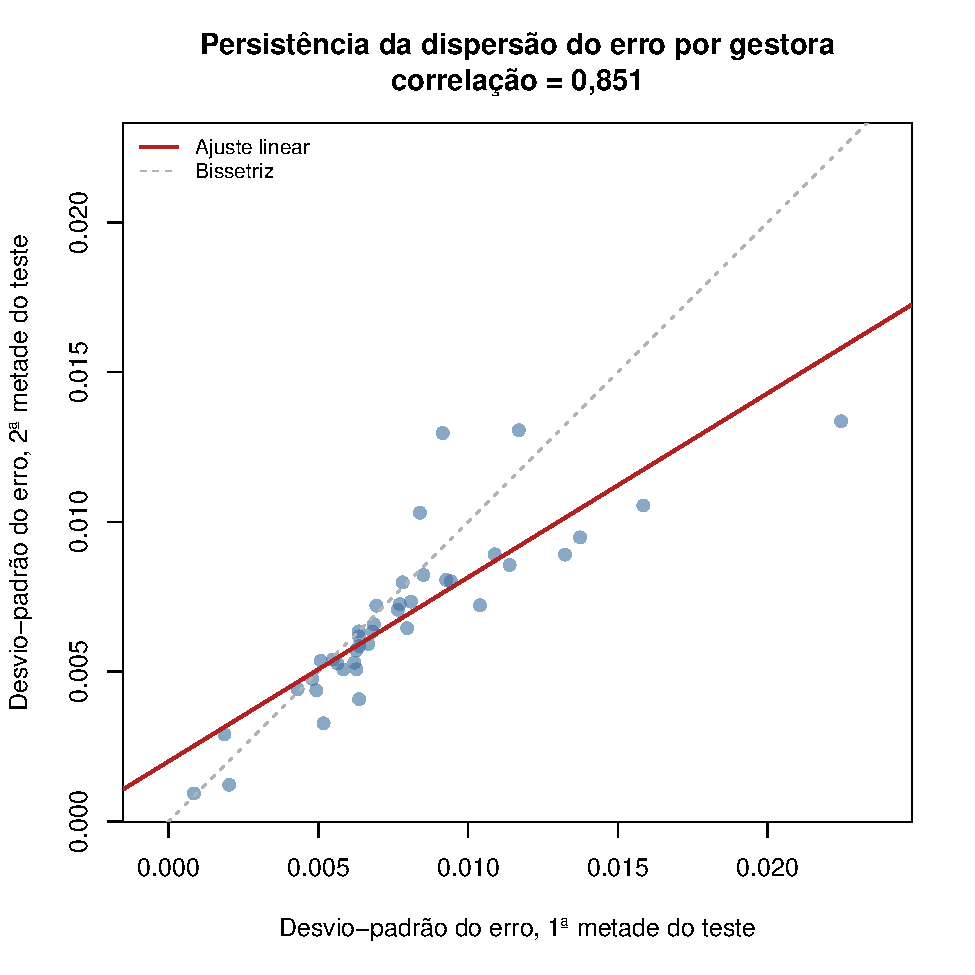
\includegraphics[width=0.55\textwidth]{fig_persistencia_dp_gestora.pdf}
\caption{Desvio-padrão do erro fora da amostra na primeira metade do período de teste, em
2020, contra a segunda metade, em 2021, por gestora. A linha tracejada é a bissetriz. Fonte:
elaboração própria a partir de dados da Comissão de Valores Mobiliários.}
\label{fig:persistencia-dp}
\end{figure}

\FloatBarrier

O que explica essa variância é, sobretudo, a concentração da carteira. Convém distinguir aqui
duas construções. A concentração do resto, definida na equação~\eqref{eq:hhi-resto}, exclui o
ativo-alvo, é medida no nível de fundo, ativo e mês, e já entra formalmente na primeira etapa
do modelo. A concentração média, usada apenas neste diagnóstico, inclui todos os ativos e é
medida no nível da gestora. A pergunta que ela responde é diferente: mesmo com a concentração
já dentro do modelo de peso, ela ainda explica o erro residual de gestoras inteiras? As
correlações bivariadas contra o desvio-padrão do erro por gestora indicam que sim, pois a
concentração média apresenta correlação de 0,65, contra 0,47 do beta médio e 0,09 do tamanho
médio. A Figura~\ref{fig:explica-variancia} mostra essas três relações.

\begin{figure}[H]\centering
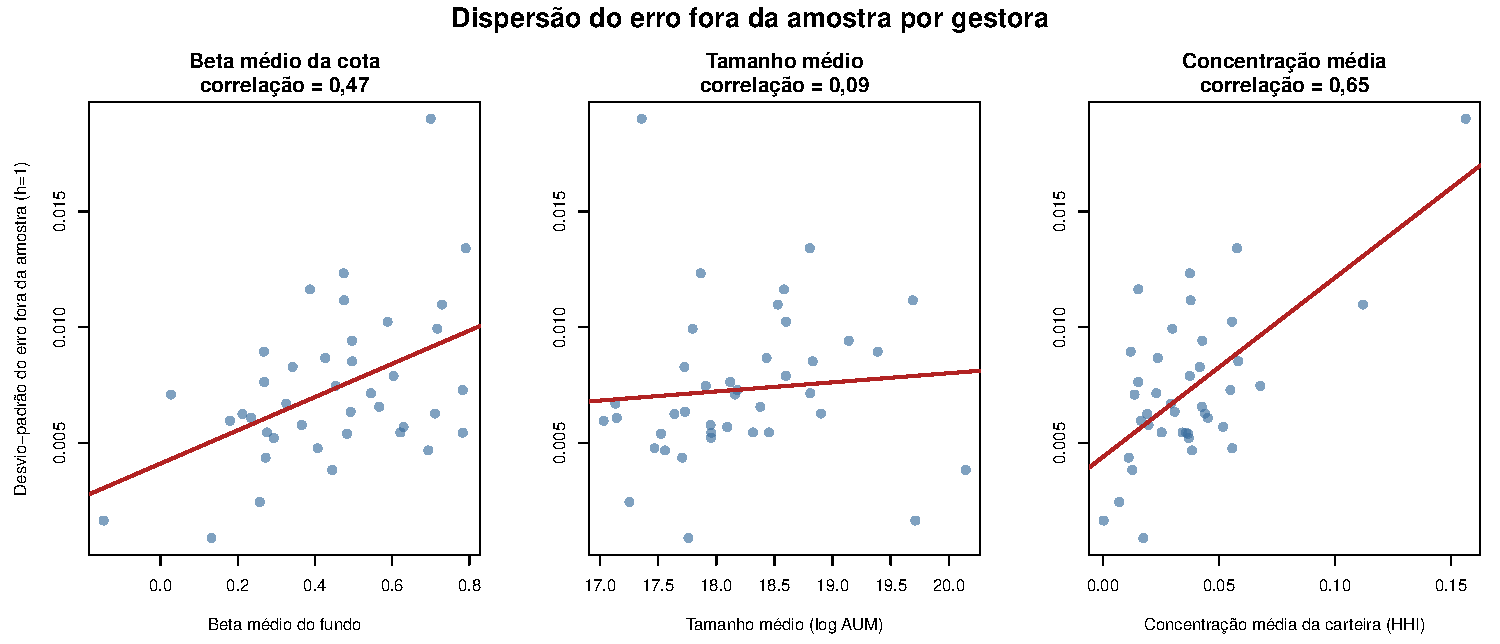
\includegraphics[width=0.95\textwidth]{fig_explica_variancia_gestora.pdf}
\caption{Desvio-padrão do erro fora da amostra por gestora contra o beta médio, o tamanho
médio e a concentração média da carteira, em 40 gestoras. Fonte: elaboração própria a partir
de dados da Comissão de Valores Mobiliários.}
\label{fig:explica-variancia}
\end{figure}

\FloatBarrier

Para isolar o efeito de cada característica, a concentração média entra numa regressão
múltipla ao lado das cinco características não relacionadas a concentração da primeira etapa,
todas medidas apenas no período de treino e, portanto, predeterminadas em relação ao desvio
do erro, que é medido apenas no período de teste:
\begin{align}
\text{dp}(\text{erro})_g = {}& \alpha + \beta_1\,\overline{\text{beta}}_g +
\beta_2\,\overline{\log(\text{patrimônio})}_g + \beta_3\,\overline{\log(\text{cotistas})}_g \notag\\
& + \beta_4\,\overline{\text{proporção de FIC}}_g + \beta_5\,\overline{\text{fluxo}}_g +
\beta_6\,\overline{\text{concentração}}_g + \varepsilon_g
\label{eq:regressao-variancia}
\end{align}

O resultado, na Tabela~\ref{tab:regressao-variancia}, é nítido. A concentração média é a
única variável estatisticamente significativa, a 1\%, e o modelo explica praticamente metade
da variação do erro entre gestoras. O fato de a concentração já estar formalmente na primeira
etapa não elimina o seu poder explicativo aqui, porque as duas regressões respondem a
perguntas distintas: a primeira etapa explica o peso de uma posição, ao passo que esta
regressão explica o erro de gestoras inteiras.

\begin{table}[h]\centering\small
\caption{Regressão do desvio-padrão do erro fora da amostra por gestora, conforme a
equação~\eqref{eq:regressao-variancia}, em 40 gestoras.}
\label{tab:regressao-variancia}
\begin{tabular}{@{}lrrc@{}}
\toprule
Variável & Coeficiente & Estatística $t$ & Significância \\
\midrule
Intercepto & $-0{,}0122$ & $-1{,}07$ & n.s. \\
Beta médio da cota & $0{,}0015$ & $0{,}55$ & n.s. \\
Tamanho médio & $0{,}0009$ & $1{,}34$ & n.s. \\
Cotistas médio & $0{,}0001$ & $0{,}18$ & n.s. \\
Proporção de fundos de cotas & $-0{,}0006$ & $-0{,}31$ & n.s. \\
Fluxo médio sobre patrimônio & $-0{,}0092$ & $-1{,}38$ & n.s. \\
Concentração média da carteira & $0{,}0736$ & $3{,}76$ & 1\% \\
\midrule
$R^2$ & \multicolumn{3}{r}{$0{,}496$} \\
\bottomrule
\end{tabular}
\caption*{\footnotesize Fonte: elaboração própria a partir de dados da Comissão de Valores
Mobiliários. A sigla n.s. indica coeficiente não significativo ao nível de 5\%.}
\end{table}

\FloatBarrier

Um refinamento para o nível de fundo e mês, em vez da média por gestora, reforça a leitura de
que a concentração é um traço permanente e não um sinal de curto prazo. A correlação
contemporânea entre concentração e erro é de 0,48, a defasada em um mês é de 0,49, valores
praticamente idênticos que afastam a hipótese de coincidência dentro do mesmo mês, mas a
correlação calculada dentro de cada fundo, após remover a sua média, cai para 0,07. Ou seja, a
concentração diferencia fundos entre si, e não meses de um mesmo fundo. Na mesma direção, o
beta médio do fundo explica 20\% da variação do erro entre os 2.039 fundos com posição e
histórico de teste suficientes.

Por fim, o ranking de dificuldade por gestora é notavelmente estável entre horizontes, como
mostra a Figura~\ref{fig:ranking}. As correlações de postos entre pares de horizontes vão de
0,91, entre um e doze meses, a 0,99, entre seis e doze meses. Isso significa que a
identificação de quais gestoras são mais difíceis de prever não é um artefato do horizonte
escolhido, e sim uma característica estável de cada casa.

\begin{figure}[H]\centering
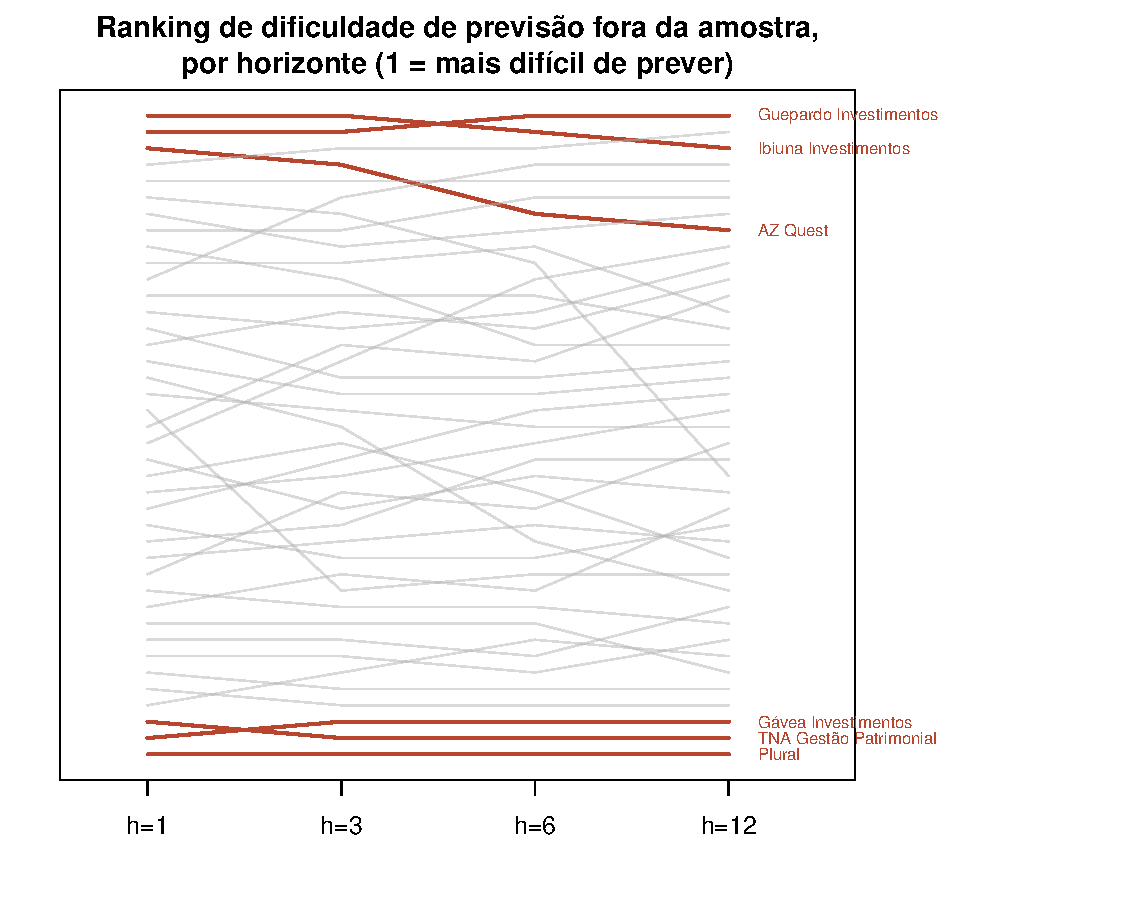
\includegraphics[width=0.75\textwidth]{fig_ranking_horizontes_slopegraph.pdf}
\caption{Estabilidade do ranking de dificuldade por gestora entre os quatro horizontes, em 40
gestoras com dado completo. Fonte: elaboração própria a partir de dados da Comissão de
Valores Mobiliários.}
\label{fig:ranking}
\end{figure}

\FloatBarrier

\begin{center}\scriptsize
\begin{longtable}{@{}lrrrrr@{}}
\caption{Raiz do erro quadrático médio fora da amostra por gestora, nos quatro horizontes,
ordenada do maior ao menor erro no horizonte de um mês. Fonte: elaboração própria a partir de
dados da Comissão de Valores Mobiliários.}
\label{tab:rmse-gestora}\\
\toprule
Gestora & Fundos & $h{=}1$ & $h{=}3$ & $h{=}6$ & $h{=}12$ \\
\midrule
\endfirsthead
\multicolumn{6}{l}{(continuação)}\\
\toprule
Gestora & Fundos & $h{=}1$ & $h{=}3$ & $h{=}6$ & $h{=}12$ \\
\midrule
\endhead
\midrule
\multicolumn{6}{r}{(continua na próxima página)}\\
\endfoot
\bottomrule
\endlastfoot
Guepardo Investimentos & 11 & $0{,}01424$ & $0{,}02305$ & $0{,}03358$ & $0{,}05649$ \\
Ibiuna Investimentos & 7 & $0{,}01331$ & $0{,}02131$ & $0{,}02492$ & $0{,}02848$ \\
AZ Quest & 22 & $0{,}01092$ & $0{,}01461$ & $0{,}01650$ & $0{,}01871$ \\
Squadra Investimentos & 15 & $0{,}01069$ & $0{,}01588$ & $0{,}02090$ & $0{,}03058$ \\
Núcleo Capital & 22 & $0{,}01037$ & $0{,}01810$ & $0{,}02468$ & $0{,}03538$ \\
Forpus Capital & 3 & $0{,}00992$ & $0{,}01436$ & $0{,}01649$ & $0{,}01666$ \\
Truxt Investimentos & 29 & $0{,}00811$ & $0{,}01263$ & $0{,}01600$ & $0{,}01978$ \\
Sharp Capital & 34 & $0{,}00800$ & $0{,}01290$ & $0{,}01713$ & $0{,}02134$ \\
ARX Investimentos & 11 & $0{,}00785$ & $0{,}01083$ & $0{,}01260$ & $0{,}01510$ \\
Kinea Investimentos & 4 & $0{,}00709$ & $0{,}01156$ & $0{,}01536$ & $0{,}01600$ \\
Constellation Asset Management & 25 & $0{,}00691$ & $0{,}01375$ & $0{,}01831$ & $0{,}02768$ \\
Opportunity & 19 & $0{,}00681$ & $0{,}01053$ & $0{,}01349$ & $0{,}01570$ \\
SPX Capital & 35 & $0{,}00614$ & $0{,}00919$ & $0{,}01174$ & $0{,}01338$ \\
Atmos Capital & 28 & $0{,}00612$ & $0{,}00999$ & $0{,}01340$ & $0{,}01711$ \\
Verde Asset Management & 14 & $0{,}00601$ & $0{,}01020$ & $0{,}01297$ & $0{,}01643$ \\
Absolute Investimentos & 7 & $0{,}00585$ & $0{,}00921$ & $0{,}01220$ & $0{,}01408$ \\
JGP & 46 & $0{,}00559$ & $0{,}00784$ & $0{,}00902$ & $0{,}01079$ \\
Daycoval Asset Management & 6 & $0{,}00557$ & $0{,}00730$ & $0{,}00726$ & $0{,}00827$ \\
Kapitalo Investimentos & 22 & $0{,}00536$ & $0{,}00580$ & $0{,}00693$ & $0{,}00818$ \\
Credit Suisse & 65 & $0{,}00533$ & $0{,}00741$ & $0{,}00859$ & $0{,}00974$ \\
Bogari Capital & 15 & $0{,}00530$ & $0{,}00925$ & $0{,}01200$ & $0{,}01575$ \\
Real Investor & 5 & $0{,}00491$ & $0{,}00919$ & $0{,}01401$ & $0{,}01742$ \\
Caixa & 31 & $0{,}00491$ & $0{,}00744$ & $0{,}00990$ & $0{,}01275$ \\
Vinci Partners & 47 & $0{,}00487$ & $0{,}00682$ & $0{,}00780$ & $0{,}00899$ \\
Claritas Investimentos & 10 & $0{,}00482$ & $0{,}00706$ & $0{,}00795$ & $0{,}00849$ \\
Bradesco Asset Management & 302 & $0{,}00445$ & $0{,}00620$ & $0{,}00736$ & $0{,}00875$ \\
BB Asset Management & 129 & $0{,}00441$ & $0{,}00671$ & $0{,}00838$ & $0{,}01022$ \\
Western Asset & 26 & $0{,}00438$ & $0{,}00701$ & $0{,}00963$ & $0{,}01253$ \\
Occam Brasil & 27 & $0{,}00430$ & $0{,}00715$ & $0{,}00831$ & $0{,}01096$ \\
BTG Pactual & 143 & $0{,}00416$ & $0{,}00629$ & $0{,}00743$ & $0{,}00911$ \\
Safra Asset Management & 155 & $0{,}00397$ & $0{,}00564$ & $0{,}00668$ & $0{,}00763$ \\
Santander Brasil Asset Management & 70 & $0{,}00394$ & $0{,}00550$ & $0{,}00630$ & $0{,}00734$ \\
Julius Baer Family Office & 62 & $0{,}00329$ & $0{,}00452$ & $0{,}00538$ & $0{,}00642$ \\
XP & 89 & $0{,}00327$ & $0{,}00478$ & $0{,}00565$ & $0{,}00748$ \\
BNP Paribas & 44 & $0{,}00324$ & $0{,}00462$ & $0{,}00561$ & $0{,}00744$ \\
Itaú & 466 & $0{,}00261$ & $0{,}00385$ & $0{,}00473$ & $0{,}00559$ \\
Dahlia Capital & 18 & $0{,}00245$ & $0{,}00422$ & $0{,}00549$ & $0{,}00631$ \\
TNA Gestão Patrimonial & 29 & $0{,}00150$ & $0{,}00216$ & $0{,}00278$ & $0{,}00384$ \\
Gávea Investimentos & 17 & $0{,}00144$ & $0{,}00265$ & $0{,}00365$ & $0{,}00472$ \\
Plural & 1 & $0{,}00050$ & $0{,}00079$ & $0{,}00104$ & $0{,}00134$ \\
\end{longtable}
\end{center}

\begin{center}\scriptsize
\begin{longtable}{@{}lrrrr@{}}
\caption{Margem do ajuste parcial sobre a previsão ingênua, em redução percentual do erro,
na mesma ordem da Tabela~\ref{tab:rmse-gestora}. Valor negativo indica que o ajuste parcial
prevê pior que a regra ingênua. Fonte: elaboração própria a partir de dados da Comissão de
Valores Mobiliários.}
\label{tab:margem-gestora}\\
\toprule
Gestora & $h{=}1$ & $h{=}3$ & $h{=}6$ & $h{=}12$ \\
\midrule
\endfirsthead
\multicolumn{5}{l}{(continuação)}\\
\toprule
Gestora & $h{=}1$ & $h{=}3$ & $h{=}6$ & $h{=}12$ \\
\midrule
\endhead
\midrule
\multicolumn{5}{r}{(continua na próxima página)}\\
\endfoot
\bottomrule
\endlastfoot
Guepardo Investimentos & $1{,}2\%$ & $1{,}0\%$ & $-0{,}1\%$ & $-1{,}3\%$ \\
Ibiuna Investimentos & $3{,}1\%$ & $6{,}8\%$ & $8{,}2\%$ & $14{,}3\%$ \\
AZ Quest & $3{,}1\%$ & $6{,}7\%$ & $9{,}5\%$ & $15{,}1\%$ \\
Squadra Investimentos & $-5{,}4\%$ & $-13{,}7\%$ & $-24{,}3\%$ & $-45{,}6\%$ \\
Núcleo Capital & $-1{,}0\%$ & $-2{,}1\%$ & $-2{,}0\%$ & $-5{,}7\%$ \\
Forpus Capital & $2{,}4\%$ & $5{,}9\%$ & $7{,}7\%$ & $11{,}5\%$ \\
Truxt Investimentos & $1{,}7\%$ & $3{,}8\%$ & $5{,}9\%$ & $13{,}1\%$ \\
Sharp Capital & $1{,}8\%$ & $4{,}6\%$ & $8{,}2\%$ & $15{,}2\%$ \\
ARX Investimentos & $2{,}1\%$ & $4{,}3\%$ & $6{,}9\%$ & $7{,}9\%$ \\
Kinea Investimentos & $1{,}7\%$ & $3{,}7\%$ & $8{,}1\%$ & $10{,}0\%$ \\
Constellation Asset Management & $-0{,}2\%$ & $0{,}6\%$ & $2{,}8\%$ & $4{,}0\%$ \\
Opportunity & $1{,}6\%$ & $3{,}8\%$ & $6{,}2\%$ & $9{,}6\%$ \\
SPX Capital & $2{,}7\%$ & $6{,}5\%$ & $10{,}5\%$ & $17{,}9\%$ \\
Atmos Capital & $0{,}2\%$ & $2{,}9\%$ & $5{,}1\%$ & $11{,}8\%$ \\
Verde Asset Management & $0{,}6\%$ & $1{,}6\%$ & $3{,}0\%$ & $-0{,}3\%$ \\
Absolute Investimentos & $1{,}8\%$ & $4{,}0\%$ & $7{,}3\%$ & $11{,}5\%$ \\
JGP & $2{,}1\%$ & $3{,}9\%$ & $4{,}8\%$ & $7{,}8\%$ \\
Daycoval Asset Management & $2{,}8\%$ & $5{,}6\%$ & $7{,}9\%$ & $12{,}3\%$ \\
Kapitalo Investimentos & $2{,}7\%$ & $5{,}8\%$ & $7{,}1\%$ & $8{,}0\%$ \\
Credit Suisse & $2{,}4\%$ & $4{,}9\%$ & $7{,}8\%$ & $13{,}8\%$ \\
Bogari Capital & $-0{,}4\%$ & $0{,}3\%$ & $0{,}9\%$ & $-3{,}2\%$ \\
Real Investor & $-1{,}4\%$ & $1{,}2\%$ & $2{,}4\%$ & $8{,}2\%$ \\
Caixa & $1{,}5\%$ & $3{,}6\%$ & $6{,}0\%$ & $8{,}3\%$ \\
Vinci Partners & $1{,}3\%$ & $3{,}0\%$ & $6{,}1\%$ & $16{,}7\%$ \\
Claritas Investimentos & $1{,}8\%$ & $6{,}1\%$ & $10{,}6\%$ & $18{,}4\%$ \\
Bradesco Asset Management & $1{,}9\%$ & $3{,}5\%$ & $4{,}5\%$ & $4{,}2\%$ \\
BB Asset Management & $1{,}0\%$ & $2{,}0\%$ & $3{,}2\%$ & $3{,}5\%$ \\
Western Asset & $1{,}1\%$ & $3{,}1\%$ & $5{,}2\%$ & $5{,}7\%$ \\
Occam Brasil & $1{,}8\%$ & $4{,}0\%$ & $6{,}8\%$ & $9{,}6\%$ \\
BTG Pactual & $1{,}1\%$ & $2{,}0\%$ & $2{,}9\%$ & $5{,}5\%$ \\
Safra Asset Management & $1{,}7\%$ & $3{,}4\%$ & $6{,}6\%$ & $14{,}2\%$ \\
Santander Brasil Asset Management & $1{,}9\%$ & $4{,}1\%$ & $5{,}4\%$ & $7{,}1\%$ \\
Julius Baer Family Office & $1{,}4\%$ & $3{,}7\%$ & $6{,}7\%$ & $10{,}1\%$ \\
XP & $-1{,}6\%$ & $-3{,}4\%$ & $-4{,}5\%$ & $-4{,}6\%$ \\
BNP Paribas & $0{,}4\%$ & $-0{,}1\%$ & $-1{,}8\%$ & $-5{,}7\%$ \\
Itaú & $1{,}9\%$ & $4{,}2\%$ & $6{,}2\%$ & $8{,}1\%$ \\
Dahlia Capital & $2{,}4\%$ & $5{,}3\%$ & $8{,}0\%$ & $10{,}2\%$ \\
TNA Gestão Patrimonial & $0{,}1\%$ & $-0{,}8\%$ & $-0{,}8\%$ & $2{,}3\%$ \\
Gávea Investimentos & $2{,}2\%$ & $4{,}2\%$ & $7{,}9\%$ & $10{,}4\%$ \\
Plural & $-2{,}4\%$ & $-3{,}7\%$ & $-2{,}8\%$ & $-6{,}1\%$ \\
\end{longtable}
\end{center}

\FloatBarrier

%==================== 6. CONCLUSÃO ====================
\section{Conclusão}
\label{sec:conclusao}

Este trabalho propôs e testou, de ponta a ponta, um modelo de fator dinâmico para o peso de
ações na carteira dos fundos de investimento brasileiros. O modelo combina uma etapa de corte
transversal, com forma funcional logística estimada célula a célula de ativo e mês, que
relaciona seis características observáveis do fundo ao peso que ele carrega, e uma etapa de
ajuste parcial que modela a velocidade com que esse peso converge ao nível implícito por
essas características. A base final reúne 2.507 fundos, 41 grupos de gestora e 512 ativos, com
8.212.294 observações entre fevereiro de 2017 e dezembro de 2021, extraídas de um universo
bruto ainda maior de 3.254 fundos e 536 ativos, e não de um recorte restrito a uma única
gestora ou a um único papel.

Na primeira etapa, o beta da cota, a concentração do restante da carteira e o número de
cotistas são as características mais consistentemente associadas a maior peso, com sinal
positivo em 88,2\%, 87,6\% e 72,8\% das 13.723 células estimadas, ao passo que o tamanho, a
condição de fundo de cotas e o fluxo de captação líquida ficam próximos da indiferença. Na
segunda, a velocidade de ajuste estimada é de 0,069 ao mês, o que corresponde a uma meia-vida
de cerca de dez meses e caracteriza uma reversão lenta, porém sistemática, ao peso-alvo. Na
terceira, o modelo estimado apenas com dados anteriores a 2020 supera a previsão ingênua de
repetir o último peso nos quatro horizontes testados, com a razão entre as raízes dos erros
quadráticos médios caindo de 0,9849 em um mês para 0,9291 em doze meses, e vence em todos os
23 meses do período de teste.

O achado que este trabalho considera mais interessante, contudo, não é o desempenho agregado,
e sim a estrutura do erro. A dificuldade de previsão é muito heterogênea entre gestoras, com
quase trinta vezes de distância entre os extremos, e essa heterogeneidade é persistente ao
longo do tempo, sobretudo na dispersão do erro, cuja correlação entre as duas metades do
período de teste é de 0,85, contra 0,73 do viés. Como o viés responde por menos de meio por
cento do erro quadrático e é praticamente incorrigível na prática, é a variância que importa,
e ela é explicada de forma robusta pela concentração da carteira. Mesmo com a concentração do
restante da carteira já formalmente dentro do modelo de peso, a concentração média da gestora
permanece a única variável significativa numa regressão que inclui todas as demais
características, com coeficiente significativo a 1\% e ajuste de 0,496. A leitura econômica é
que a previsibilidade da carteira de um fundo é, em boa medida, uma função do seu estilo de
concentração: casas que concentram são estruturalmente mais difíceis de prever, e não apenas
mais voláteis em algum período específico.

Quatro limitações merecem registro. A primeira é que parte substancial da variância do erro
fora da amostra permanece sem explicação pelas seis características observáveis, uma vez que
o beta médio explica 20\% da variação do erro entre fundos e a regressão múltipla por gestora
explica cerca de metade da variação entre gestoras, o que sugere a presença de fatores
específicos de fundo, como estilo, restrições de mandato e liquidez da carteira, não
capturados neste desenho. A segunda é que o recorte temporal da amostra final, de fevereiro
de 2017 a dezembro de 2021, reflete a disponibilidade de dado público com qualidade
suficiente para a limpeza descrita na Seção~\ref{sec:dados}, de modo que estender a análise a
um período mais recente fica como trabalho futuro. A terceira diz respeito à identificação: o
beta da cota é medido com dado até o fechamento do próprio mês da observação, e não do mês
anterior como as outras cinco características, o que não utiliza informação futura mas abre
uma via de endogeneidade mecânica, já que o retorno da cota depende em parte das posições que
o modelo procura explicar. A quarta é que o mecanismo de ajuste parcial, como qualquer modelo
dessa família, incluindo os citados na Seção~\ref{sec:revisao}, tem a distância até o alvo e a
variação do peso compartilhando o termo do peso corrente por construção, o que favorece
mecanicamente uma estimativa positiva da velocidade de ajuste mesmo sob ruído de medição
transitório, sem que este trabalho consiga isolar quanto dos 0,069 estimados é ajuste genuíno
e quanto é esse artefato.

Três extensões parecem naturais. A primeira é permitir que a velocidade de ajuste varie entre
gestoras ou entre classes de fundo, em vez de impor um único parâmetro comum, o que os
resultados de heterogeneidade desta seção sugerem ser empiricamente relevante. A segunda é
incorporar características de mandato e de liquidez da carteira, hoje ausentes do conjunto de
seis variáveis, com o objetivo de capturar a parcela da variância do erro que permanece sem
explicação. A terceira é estender o painel para além de 2021, o que permitiria avaliar se os
padrões documentados aqui sobrevivem a um regime de juros e de fluxo bastante distinto do que
vigorou no período estudado.

% ======================================================================
\bibliography{referencias}

\end{document}
